\documentclass[11p]{article}
% Packages
\usepackage{titlesec}
\usepackage{hyperref}
\usepackage{amsmath}
\usepackage{graphicx}
\usepackage{fancyheadings}
\usepackage[swedish]{babel}
\usepackage[
    backend=biber,
    style=authoryear-ibid,
    sorting=ynt
]{biblatex}
\usepackage[utf8]{inputenc}
\usepackage[T1]{fontenc}
%Källor
\addbibresource{references.bib}
\graphicspath{ {./images/} }

% Lite variabler
\def\email{endo.axelsson@ga.ntig.se}
\def\foottitle{PMmall}
\def\name{Endo Axelsson}

\title{PMmall \\ \small Gymnasiearbete}
\author{\name}
\date{\today}

\begin{document}

% fixar sidfot
    \lfoot{\footnotesize{\name \\ \email}}
    \rfoot{\footnotesize{\today}}
    \lhead{\sc\footnotesize\foottitle}
    \rhead{\nouppercase{\sc\footnotesize\leftmark}}
    \pagestyle{fancy}
    \renewcommand{\headrulewidth}{0.2pt}
    \renewcommand{\footrulewidth}{0.2pt}

% i Sverige har vi normalt inget indrag vid nytt stycke
    \setlength{\parindent}{0pt}
% men däremot lite mellanrum
    \setlength{\parskip}{10pt}

    \maketitle

    \begin{document}

        \begin{titlepage}
            \centering

            \vspace*{1cm}

            % Title and subtitle are enclosed between two rules.
            \rule{\textwidth}{1pt}

            % Title
            \vspace{.7\baselineskip}
            {\huge \textbf{En effektivare hjärna}}

            % Subtitle
            \vspace*{.5cm}
            {\LARGE Jämförandet mellan den kognitiva förmågan utan och med musik  }

            \rule{\textwidth}{1pt}

            \vspace{1cm}

            % Set this size for the remaining titlepage.
            \large

            % Authors side by side, using two minipages as a trick.
            \begin{minipage}{.5\textwidth}
                \centering
                Endo N. Axelsson \\
                {\normalsize \url{Endo.axelsson@elev.ga.ntig.se}}
            \end{minipage}%

            \vspace{3cm}

            % Report logo.
            
\includegraphics[width=.7\textwidth]{../images/nti_logo.png}

            \vfill

            % University and date information at the bottom of the titlepage.
            NTI Gymnasiet Umeå \\
            Teknikprogrammet\\
            Gymnasiearbete\\
            Datum: \today \\
            Handledare: Simon Karlsson
        \end{titlepage}


        \tableofcontents


    \section{Introduktion}
    Denna undersökning handlar om hur den kognitiva förmågan och arbetsminnet presterar med samband till musiken.
    Musik som på så sätt är bekant eller lätt att återkalla kan lugna ner stressnivån för att med fördel plocka upp information enklare.
    Det som undersökts är om musiken med hjälp av ett memory spel kan hålla informationen som plockas upp aktuellt i minnet.
    Är musiken en underlättande metod för den kognitiva förmågan.
    Jämväl om den hjälper inlärningen och ökar motivationen.
    Kognitiva förmågan som begrepp handlar om hur hjärnan under en kort period tar upp information medvetet.
    För att sedan lagra det, bearbetar och plocka fram informationen för senare scenarion.
    Inom studier så är användningen av musiken en studieteknik som används för att dämpa ljud runtom och få en mer passande atmosfär.
    Föruttsätningen blir att det blir mer fokus på arbetet.


    \section{Syfte och frågeställning}
    Detta är ett arbete med syftet av att undersöka och förstå interaktionen mellan de kognitiva funktionerna och ljud.
    Genom att studera och notera detta ämne kan man bättre förstå om musiken kan användas som ett verktyg för bättre koncentration, eller om det är ett störningsmoment för fokuset.
    Med analyserad data från resultaten och ett uträknad chi-två-test ska arbetet kunna svara på följande frågor.

    \begin{itemize}
        \item Hur påverkar musiken arbetsminnets prestanda och kapacitet under given uppgift?
        \item Vad har musiken för effekt på den kognitiva förmågan, till skillnad från utan?
    \end{itemize}

        \section{Bakrund}
    Hörlurar med ljud som spelas i öronen blir ett alltmer uppskattat val gällande studieteknik.
    Ett effektivt sätt att blockerar ut allt oljud runtomkring och ersätter det med harmoniska ljud som lugnar ner hjärnans stressnivå istället.
    En aspekt där folk tycker att musiken höjer dopaminet, vilket också översätts till att humöret blir bättre.
    Det resulterar till att hjärnan får mer energi och blir bättre inställd för arbete.
    Motivationen för att ta emot fakta blir större.
    Denna studie undersöker hur information lagras i minnet i sammanhang med musik och om man kan utnyttja det som en hjälpmedel för att återkalla minnerna.
    Som \textcite{Effectsmusic} presenterar i deras artikel, så är det som när väldigt unga barn blir inlärda med hjälpmedel som musiken.
    Låtar som Alfabetssången och tvätta händerna är bland de vanligaste.
    Det lär in barn alfabetet och att man ska tvätta händerna med en glad och en lätt igenkänlig melodi.
    Därtill finns det musik videor där dem visuellt associerar det som visas på skärmen med ett ord eller meningar.
    Exempel på saker som buss, färger, djur och mera.
    Lyssnar man om låtarna flertal gånger så får hjärnan små signaler från tidigare tillfällen och på så sätt återkalla det som är kopplat till det specifika situationen.
    Mera upprepande innebär att informationen blir alltmer aktuella och bekantare för minnet att hålla kvar.

    \subsection{Arbetsminnet}

    \begin{figure}
        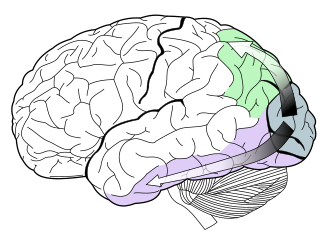
\includegraphics[width=0.6\textwidth]{../images/brain.png}
        \caption{Figur 1: caption. }
    \end{figure})


    Arbetsminnet är en central komponent i den kognitiva förmågan.
    Det är en process där hjärnan medvetet plockar fram och manipulerar relevanta information beroende på olika scenarion.
    Händelsen stimulerar hjärnan och får den att selektivt välja minnen som passar in.
    Människans minnessystem består förenklat av tre aspekter.


Hjärnans olika delar


    Med konstant upprepning och repetition så kan du manipulera minnet så att de sitter bättre.

    Men genom musiken ska minnet få fram en ett mer stabilt och sekvent arbete,utan att fokuset bryts av oljud.
    På så sätt få en mentalt lugnare miljö  för att lagra det visuella och informativa.

    BILD

    Hjärnan har flertal regioner inom sig där olika minnen lagras.
    Figur 1 visar de olika regionerna

    SPARA. Noise är en del av varje musikalisk signal och få instrument ger ifrån sig ljud utan att
    samtidigt ge ifrån sig noise.
    Detta innebär att mycket musik inte kan finnas utan närvaron av
    noise.
    Samtidigt påpekar Hegarty (2011) att noise, framställt som musik, inte kan finnas
    utan de lagar, strukturer och regler som musik innebär.
     Noise som musikaliskt uttryck
    bygger på att det måste stå som en motsats till musik.
        Därför kan inte heller noise finnas utan musik.
     De två fenomenen är beroende av varandras existens för att själva kunna


Känslomässiga tillstånd
        dämpa bakrundsljud

        Det är inte ofta nämnt att minnet som lagras är begränsat och temporär som den är.
        Kapaciteten kan överbalast och på så sätt begränsan lagringen.
        Detta är relevant eftersom belastningen fördelas annorlunda när den plockar upp ljud.

        ANTECKNING: WORKIBG MEMORY
        https://legacy.cs.indiana.edu/~port/HDphonol/Baddely.wkg.mem.Science.pdf
        engle randall Working memory, short-term memory, and general fluid intelligence: A latent-variable approach pdf

        \subsection{Visuella memory}
    Visuella memory är förmågan som tillåter en att bearbeta, återkalla och lagra det visuella från omgivningen.
    Det information som synen tar in skickas vidare till hjärnan.
    Minnet består av flera delar varav några är korttidsminnet och långtidsminnet.
    Korttidsminnet är det det minnet som är temporärt.
    Medans långtidsminnet kan både lagrar och återkallar visell information under en längre tid.
    Det uppnås genom att manipulera information som tagits emot.

    ??
    Specifikt så hamnar de i Posterior parietal cortex, vilket är en av de fyra stora delarna i hjärnan för att den ska fungera.
    Posterior parietal cortex uppfattas som funktionen för uppmärksammhet, arbetsminne och det visuella bilderna som ligger i minnet.
    Det är också det som gör så att vi kan planera vad nästa steg ska vara och kontrollera.
    \textcite{Capacitylimit}


    \subsection{Manipulering av information}
    Definitionen av att manipulera information är att kunna styra och kontrollera det med träning.
    Det finns flertal sätt att manipuleras minnet.
    Att komma ihåg något under en längre tid är en process där du konstant repeterar information så att fastnar längre.


    Memory spelet ger  är en uppgift , det inkluderar faktorer där arbetsminnet testas under ett moment...



    \section{Metod}
    I denna undersökning så kommer en grupp av personer individuellt bli indelad i två olika testgrupper: A och B, för att avgöra om musik faktist förbättrar arbetsminnet.
    Genre på musik är en faktor gällande arbetsminne, så de som är i grupp A får hörlurar där klassiskt musik spelas medans grupp B gör undersökningen ljudlöst.
    \newline För att avgöra detta så används ett memory spel som ett verktyg.
    I detta fall så ska memory spelet visa 24 styckna kort med olika bilder på, korten visas i 15 sekunder innan dem vänds.
    \newline Alla kort ligger på samma position för alla, för att det ska ge ett så rättvist resulalt så möjligt och minska slumpäss faktorn för varje test.
    Målet är att komma ihåg så många kort som möjligt och med hjälp av musiken länka det visuella till ljud.
    Arbetet utförs enskilt för att mäta hur mycket varje individ kommer ihåg utan någon påverkan av andra.

    \subsection{Memory spel}
    Korten är skapad i Indesign, där en kortmall med 24 rutor skapades.
    Varje ruta har en vit bakrund och frukt ikonerna är png, innebär att bakrunden är transparent.
    Frukt ikonerna las in i mallen 2 och 2 för varje par, tills hela blev komplett.
    Samma  mall kopierades i samma dokument för att göra baksidan.
    Exakt samma placering fast att rutorna hade NTI loggan.
    Filen sparades och konverterades till en pdf-fil där den sedan skrevs ut dubbelsidigt på ett tjockt papper.
    Pappret laminerades och klippdes ut var för sig.


    \subsection{Process}
    Testet inleds med att presentera kort för deltagaren vad arbetet handlar om.
    Introt ska klargöra varför detta utförs och vad målet med undersökningen är.
    Sedan blir deltagaren indelade en av två grupper, A eller B för att därefter få materialen som krävs för respektiv grupp, hörlurar för de i grupp A.
    Innan testet faktist börjar och för att det ska bli så riskfritt så möjligt så kommer instruktionerna precis innan.
    Det innehåller spelets innehåll, regler och vad målet är med det.
    Medans spelkorten sätts upp så får deltagaren ett annat spelkort vilket agerar som uppvärmning för hjärnan.
    Är deltagaren i test-grupp A så tillägs hörlurar med musik.
    väl klar med kortens uppställning så frågar jag om personen är klar och redo för att göra testet.
    Vid spelets start så visas kortet i 15 sekunder, efter tiden så vänds spelkorten.
    Under spelets gång så antecknas deltagarens drag i respektiv grupp och antalet fel.
    \newline Under en begränsad tid på max 5 minuter så bör deltagaren vara klar med spelet.
    Det är 24 kort totalt och med hälp av att korten visar sig 15 sekunder i början av spelets gång, så ska deltagarna para ihop så många par så möjligt med så lite fel så möjligt innan tiden tar slut.
    Då spelets gång är klar oavsett om det är för att tiden tog slut eller att man parat klart alla så avslutas det.
    När deltagaren är klar så är all resultat antecknad för senare uträkning.
    Beräkningarna ska sedan visa om vilken grupp som har presterat bättre än den andra.

    \subsection{Intro}
     Det som sägs till deltagaren är viktigt för att alla ska ha rättvis och likadan process.
     Följande information sägs till varje deltagare.
     "Som snabb bakgrund så utförs detta arbete för att undersöka om musiken har en positiv eller negativ påverkan på det visuella minnet.
     Jag kommer att visa en bild av kortleken där man får se hur de är placerade med bilderna uppvänd.
     Du har 15 sekunder på dig att memorera, efter så är det bara att börja vända och hitta paren."



    \subsection{Urval}
    Selektionen av detta arbete består av medelstora klasser på gymnasie nivå.
    Deltagande elever kommer att vara i åldrarna mellan 16 till 18 år.
    Detta är relevant efersom åldersgruppen i gymnasieskolor använder mycket digital läromedel vilket påverkar koncentrationsförmågan på olika sätt.
    Flertal skolor är osäkra om det faktist hjälper eleverna eller om det bara är en annan störningsmoment.
    Åldrarna i gymnasiet är målgruppen där detta är som mest relevant.
    Detta skapar ett tillfälle för en studie som kan säga på ett ungefär om läromedlet är positiv för inlärningen.


    \subsection{Etik}
    Valet att delta är helt valfritt och de som inte vill vara med behöver inte det.
    Datan som samlas in är helt anonymt och visar ingen uppgiven namn.
    Resultaten består endast av siffror, procent och om test-personen var i grupp A eller grupp B.
    Det enda undantaget är test klassen namn, vilket krävs för att kunna identifera och gruppera varsifrån data samlats in ifrån.

        \section{Resultat}
        Undersökningen hade totalt 20 personer som frivilligt ställde upp, varav alla var mellan åldrarna 16 till 18 år i gymnasiet.

        Grupperna för A och B var jämnt fördelade med 10 styckna i respektive.
        Alla 20 personer
        Från datan som samlades in gjordes tre tester.


        Lägg till (utfört tre tester) Medel spridning och ttest.
        Skriv ner resultatet under varje rubrik.
        först som flytande text
        (vadhar du observerat) och sedan lägg till diagram/Tabeller/grafer/beräkningar

        \subsection{Medelvärde}

        Det som observerades var att avståndet i medelvärde för grupp A och B var minimal.
        2 drag skilde sig.
        Uträkningen av medelvärdet utfördes genom att använda varje grupps medeldrag och dela det med antalet.
        Detta gjordes för båda grupperna som sedan sattes in i ett diagram för presentation.
        \begin{figure}
            \includegraphics[width=0.9\textwidth]{../images/Medelvärde.png}
            \caption{Diagram av medelvärderna för grupp A (Blå) och grupp B (Röd)}
        \end{figure}

        \subsection{Spridningsdiagram}
        Med hjälp av värderna från figur ... valdes spridningdiagram för att se spridning mellan grupp A och B
        Det man ser är att grupp A har bättre resultat men har en större utspridning.
        Grupp B som utförde testet utan musik fick generellt sämre resultat men svaren var mer konsekvensa.

        \begin{figure}
            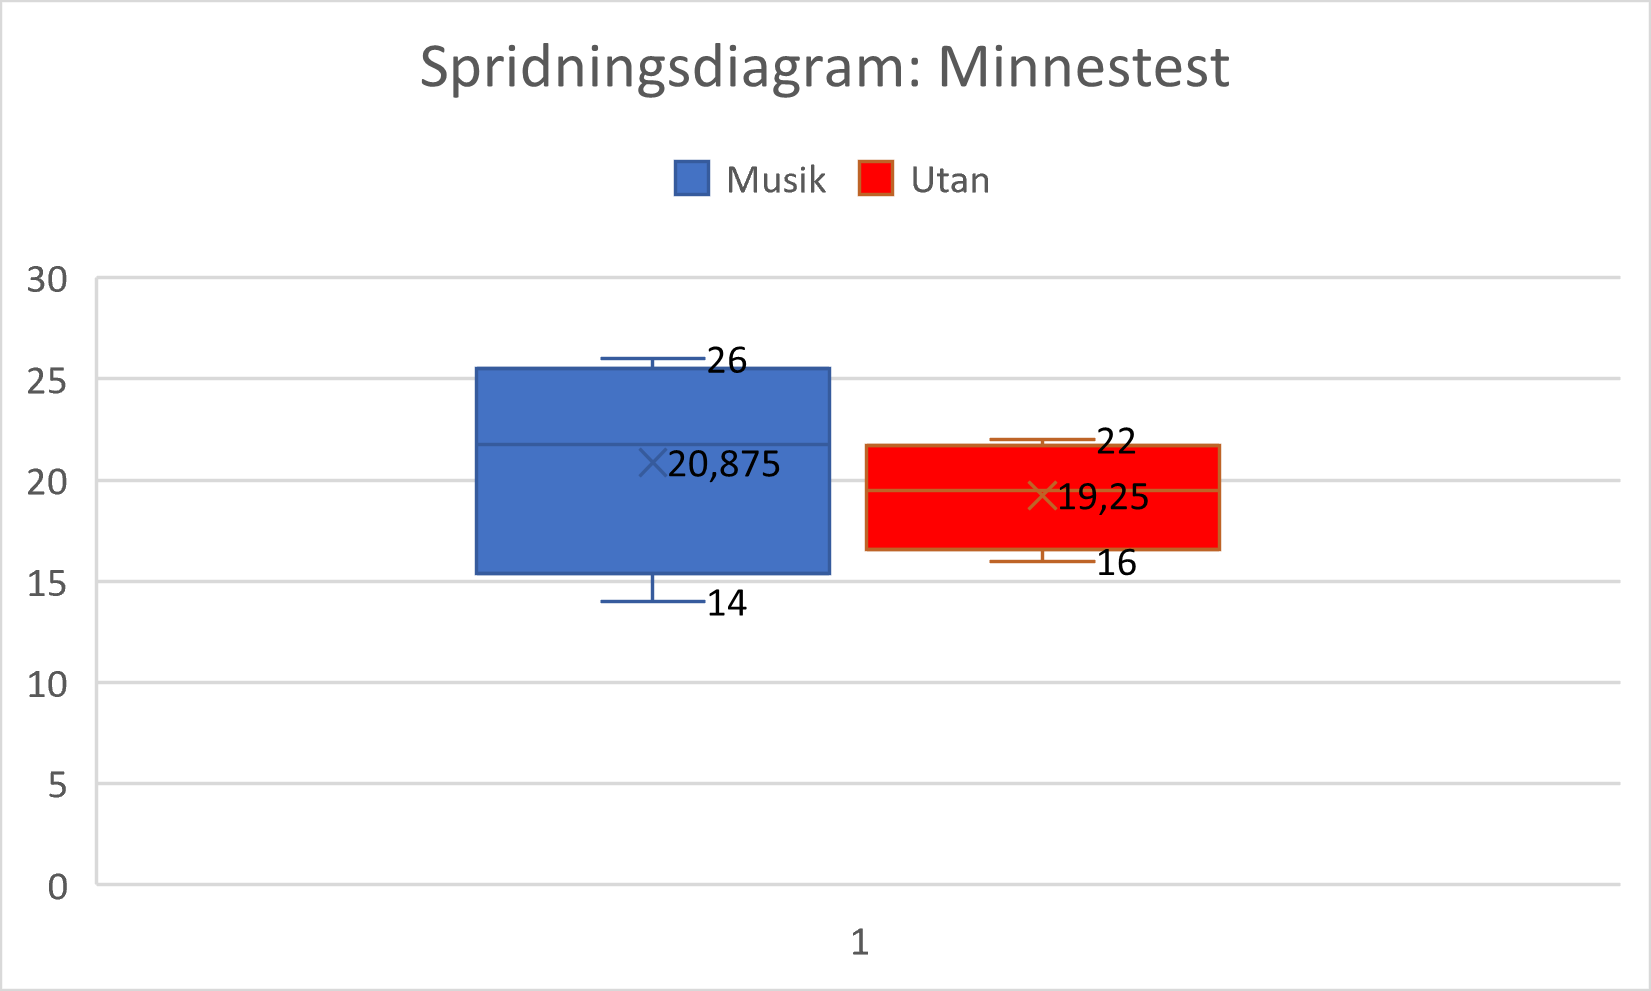
\includegraphics[width=1\textwidth]{../images/spridningsdiagram.png}
            \caption{Spridningsdiagram }
        \end{figure}

        \subsection{Chi-två test}

        Om X är större än värdet 5 procent så kan nollhypotesen förkastas.
        \begin{figure}
            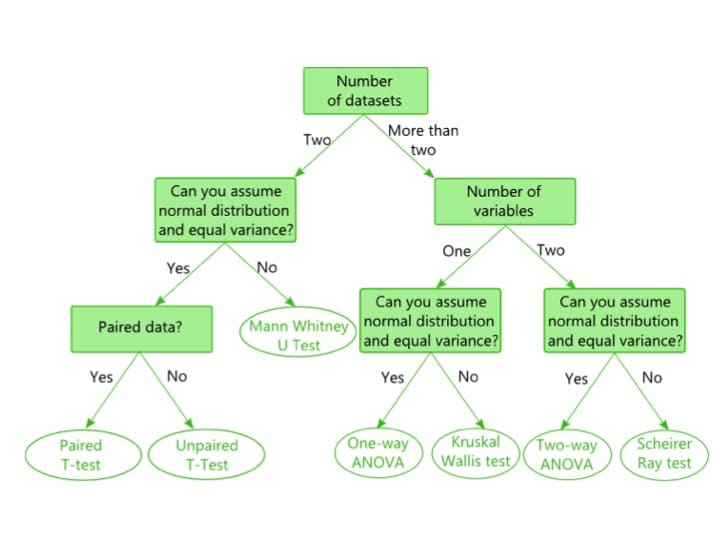
\includegraphics[width=0.8\textwidth]{../images/data.jpg}
            \caption{Figur 1: caption. }
        \end{figure}

        \subsection{Analys av data}
    Jämförelser mellan grupperna, vad är de som jämförs?

    Alla kommer att ha 12 rätt men antalet drag kommer att varieras

    lådagram (presentera)- medelvärde- t test

    \begin{figure}
        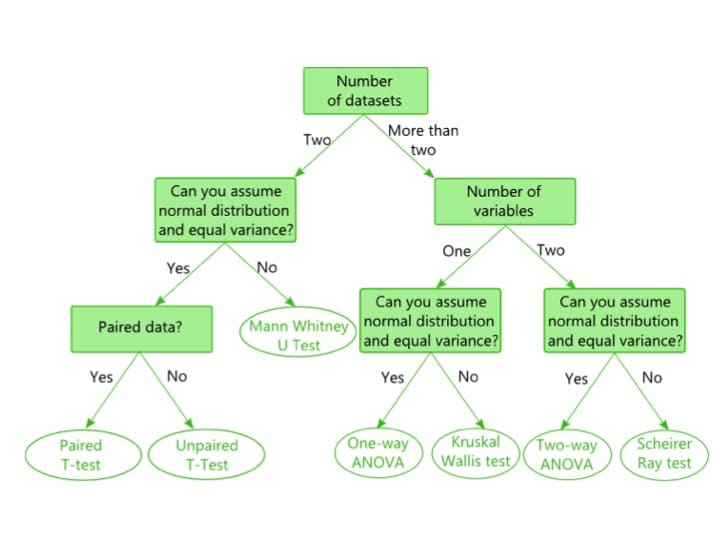
\includegraphics[width=0.8\textwidth]{../images/data.jpg}
        \caption{Figur 1: caption. }
    \end{figure}

    https://bitesizebio.com/19298/comparing-two-sets-of-data/


    \section{Diskussion}
    Utifrån det data som samlats in och presenterats så syns skillnaden tydligt.
    Enligt studiens slutgiltiga resultat så


    Det som finns att tänka på är de olika faktorerna som påverkar resultat.
    Vilken genre på musiken kan kopplas annorlunda för olika personer och
    Faktorer som kan anting försämra eller förbättra detta, som vilken genre musiken är eller vilken nivå deltagarens koncentrationsnivå ligger på.


    %Spelen som redan existerade på nätet var för slumpässiga för att få ett rättvist och en stabil resultat.
    %det fel som inte var passande för undersökningen: korten blandades om för varje omgång som spelades och visades inte i början, vilket gör att de första kortvändingarna ökar felmarginalen.
    %Så för att undvika detta så ska
    %färger

        \subsection{Faktorer som påverkar}
        Omständigheterna vid skapandet av det digitala memory spelet gjorde att arbetet utfördes analogt.
        Det analoga undersökningen minimerade antalet personer som testas samtidigt.
        Varje deltagare behövde sina egna intro för varje test som utfördes och det konsumerade tid.
        Antalet som testades fick därför minska.


        \subsection{Svar på frågeställningen}


    \subsection{Slutsats}

störningsmoment?
Fokuset hamnar på fel aspekt när musik spelas
    \printbibliography

    \end{document}
